\section{Auswertung}
\subsection{Daten}
Hier sind die Daten der verwendeten Spulen
aufgelistet.\\
\noindent Ringspule mit Luftspalt:\\
\begin{align*}
  &\text{Breite Luftspalt:}\; d=3mm &\text{Windungszahl:}\; n=595
\end{align*}
\noindent Helmholzspulen:\\
\begin{align*}
  &\text{Windungszahl:}(je)\; n=100 &\text{Spulenbreite:}\; b=33mm\\
  &\text{Durchmesser:}\; d=125mm
\end{align*}
Lange Spule:\\
\begin{align*}
  &\text{Windungszahl:}\; n=300 &\text{Länge:}\; l=16cm\\
  &\text{Durchmesser:}\; d=41mm
\end{align*}
Kurze Spule:\\
\begin{align*}
  &\text{Windungszahl:}\; n=3400 &\text{Länge:}\; l=10cm\\
\end{align*}
\subsection{Hysteresekurve}
\noindent Um die Hysteresekurve einer Ringspule mit
Luftspalt zu bestimmen, wurden die in Tabelle
\ref{tab:tabelle1} dargestellten Messwerte in einem
Diagramm aufgetragen. Dieses Diagramm ist ist Abbildung
\ref{fig:plothys} dargestellt.
\begin{table}[H]
  \centering
  \caption{Messwerte der Wärmepumpe}
  \label{tab:tabe1}
    \begin{tabular}{S S S S S S}
    \toprule
    $ t  \: / \si{\second} $ & $ p_a \: / \si{\bar} $ & $ p_b \: / \si{\bar} $ &
    $ T_1 \: / \si{\kelvin} $ & $ T_2 \: / \si{\kelvin} $ & $ P \: / \: \si{\watt} $\\
    \midrule
    0 & 5.0 & 5.0 & 293.65 & 293.65 & 0 \\
    60 & 4.7 & 6.0 & 294.15 & 293.55 & 115 \\
    120 & 4.4 & 6.4 & 295.15 & 293.15 & 118 \\
    180 & 4.5 & 6.9 & 296.35 & 291.95 & 122 \\
    240 & 4.6 & 7.0 & 297.55 & 290.95 & 125 \\
    300 & 4.6 & 7.0 & 298.85 & 289.95 & 125 \\
    360 & 4.5 & 7.2 & 300.05 & 289.15 & 123 \\
    420 & 4.4 & 7.4 & 301.15 & 288.45 & 123 \\
    480 & 4.3 & 7.8 & 302.35 & 287.65 & 122 \\
    540 & 4.2 & 8.0 & 303.55 & 286.95 & 122 \\
    600 & 4.2 & 8.1 & 304.65 & 286.25 & 121 \\
    660 & 4.1 & 8.3 & 305.75 & 285.55 & 121 \\
    720 & 4.0 & 8.5 & 306.75 & 284.95 & 121 \\
    780 & 4.0 & 8.8 & 307.75 & 284.35 & 121 \\
    840 & 3.9 & 9.0 & 308.75 & 283.75 & 121 \\
    900 & 3.8 & 9.1 & 309.65 & 283.15 & 121 \\
    960 & 3.8 & 9.2 & 310.55 & 282.55 & 122 \\
    1020 & 3.8 & 9.5 & 311.45 & 282.05 & 122 \\
    1080 & 3.7 & 9.8 & 312.25 & 281.55 & 122 \\
    1140 & 3.7 & 10.0 & 313.05 & 281.15 & 122 \\
    1200 & 3.7 & 10.0 & 313.9 & 280.65 & 122 \\
    1260 & 3.6 & 10.2 & 314.65 & 280.25 & 123 \\
    1320 & 3.6 & 10.3 & 315.35 & 279.85 & 123 \\
    1380 & 3.6 & 10.6 & 316.15 & 279.45 & 124 \\
    1440 & 3.6 & 10.8 & 316.85 & 279.15 & 124 \\
    1500 & 3.6 & 11.0 & 317.55 & 278.75 & 124 \\
    1560 & 3.6 & 11.1 & 318.25 & 278.55 & 124 \\
    1620 & 3.6 & 11.2 & 318.95 & 278.25 & 125 \\
    1680 & 3.5 & 11.4 & 319.55 & 277.95 & 125 \\
    1740 & 3.5 & 11.5 & 320.15 & 277.65 & 125 \\
    1800 & 3.5 & 11.7 & 320.75 & 277.45 & 125 \\
    1860 & 3.5 & 11.9 & 321.35 & 277.25 & 125 \\
    1920 & 3.5 & 12.0 & 321.95 & 277.05 & 125 \\
    1980 & 3.5 & 12.1 & 322.45 & 276.95 & 125 \\








      \bottomrule
    \end{tabular}
\end{table}

\begin{figure}[H]
  \centering
  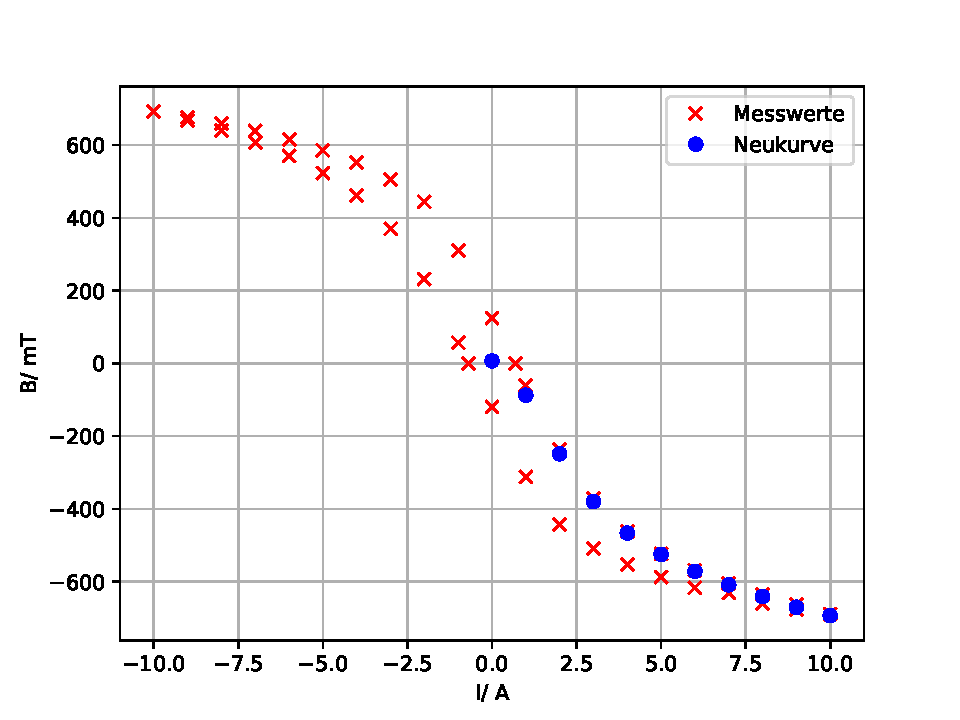
\includegraphics[height=8cm]{plothys.pdf}
  \caption{Hysteresekurve einer Ringspule mit Luftspalt.}
  \label{fig:plothys}
\end{figure}
\noindent An Abbildung \ref{fig:plothys} und auch an den
Messwerten
aus Tabelle \ref{tab:tabelle1} kann die
Sättigungsmagnetisierung $B_{S}$, die Remanenz
$B_{r}$ für $I=0$ sowie die Koerzitivfeldstärke
$H_{k}$ abgelesen werden.
Die Beträge der Werte werden nach der Formel
\begin{equation}
  \bar{x}=\frac{1}{N}\sum_{1}^N x_{i}
  \label{eqn:mittel}
\end{equation}
gemittelt, dabei bezeichnet $N$ die Anzahl der zu
mittelnden Werte. Wenn die Messwerte aus Tabelle \ref{tab:tabelle1} verwendet
werden, kann der dazugehörige Fehler über
\begin{equation}
  \Delta\bar x = \frac{1}{N}\sqrt{\frac{1}{N-1}\cdot\sum_{1}^N (x_{i}-\bar x)^2}
\end{equation}
berechnet werden.
Für die Sättigungsmagnetisierung und
Remanenz ergeben sich folgende Werte:
\begin{align*}
  B_{S} &=\SI{691,5(12)}{\milli\tesla} \\
  B_{r} &=\SI{121.3(22)}{\milli\tesla}
\end{align*}
Die Koerzitivfeldstärke $H_{k}$, kann aus den Werten in
Tabelle \ref{tab:tabelle1} wie folgt berechnet werden:
\begin{equation}
  H_{k}=\SI{0,7}{\ampere}-(\SI{-0,7}{\ampere})=\SI{1,4}{\ampere}.
  \label{eqn:koerzitiv}
\end{equation}


\subsection{Helmholzspulen}
\noindent Die Messwerte für die erste Messung mit $I=2A$
sind in Tabelle \ref{tab:tabelle3} dargestellt.
\begin{table}
  \centering
  \caption{Messwerte für den ersten Doppelspalt.}
   \begin{tabular}{S S| S S | S S}
    \toprule
    $x/\; \si{\mm}$& $A/\;\si{\nA}$ &
    $x/\; \si{\mm}$& $A/\;\si{\nA}$ &
    $x/\; \si{\mm}$& $A/\;\si{\nA}$ \\
    \midrule

    15.0& 4.6& 23.0& 25.0& 29.5& 6.0\\
    15.5& 4.2& 23.5& 30.0& 30.0& 5.3\\
    16.0& 4.0& 24.0& 35.0& 30.5& 4.9\\
    16.5& 4.0& 24.25& 36.0& 31.0& 4.7\\
    17.0& 4.4& 24.5& 37.0& 31.5& 4.4\\
    17.5& 5.5& 24.75& 38.0& 32.0& 4.2\\
    18.0& 6.6& 25.00& 37.0& 32.5& 3.8\\
    18.5& 7.7& 25.25& 36.0& 33.0& 3.6\\
    19.0& 8.2& 25.5& 36.0& 33.5& 3.2\\
    19.5& 8.4& 26.0& 33.0& 34.0& 3.2\\
    20.0& 8.4& 26.5& 28.5& 34.5& 3.2\\
    20.25& 8.4& 27.0& 23.0& 35.0& 3.3\\
    20.5& 8,7& 27.5& 18.0& 35.5& 3.4\\
    21.0& 9.8& 28.0& 13.5& 36.0& 3.5\\
    21.5& 12.0& 28.5& 10.0\\
    22.0& 15.0& 29.0& 7.8\\
    22.5& 20.0& 29.25& 6.7\\


   \bottomrule
  \end{tabular}
  \label{tab:tabelle3}
\end{table}

Die Messwerte für den Innenbereich der Spulen und den
Außenbereich wurden getrennt in einem xB-Diagramm
aufgetragen und mit der Theoriekurve aus Gleichung \ref{eqn:Helmholtz}
verglichen. Die Diagramme sind in Abbildung
\ref{fig:Helmholz1} und \ref{fig:Helmholz1I}
dargestellt. Dabei muss berücksichtigt werden, dass die
Theoriekurve den Mittelpunkt zwischen den Spulen als
Nullpunkt annimmt, sich der der Nullpunkt der
Messwerte jedoch an Rand der ersten Spule befindet.
\begin{figure}[H]
  \centering
  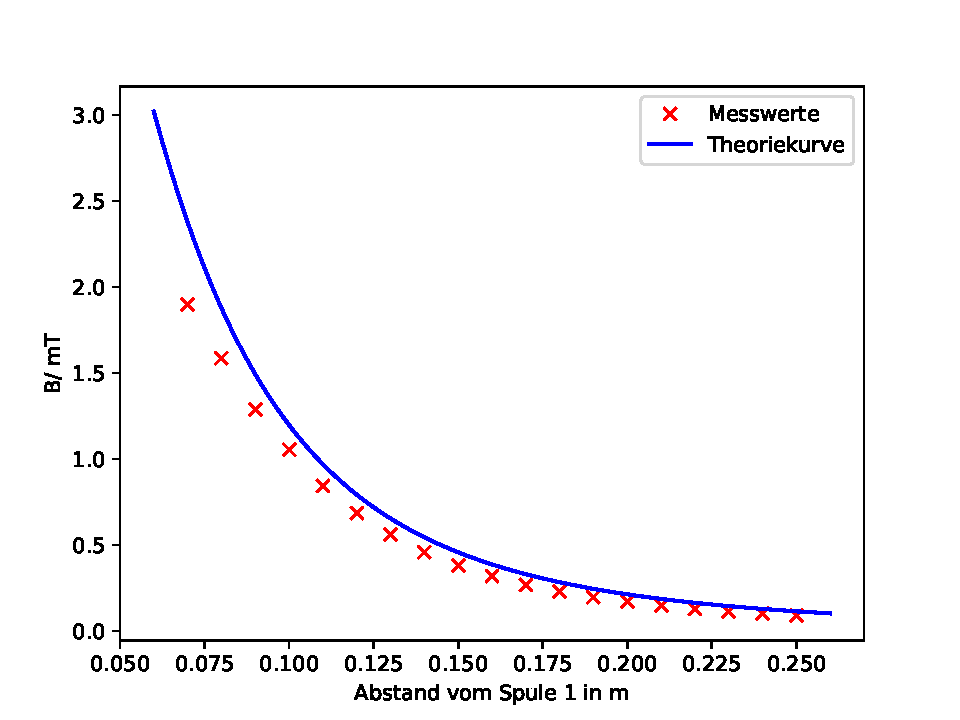
\includegraphics[height=8cm]{Helmholz1.pdf}
  \caption{xB-Diagramm des Außenbereiches eines
  Helmholzspulenpaares im Vergleich zur Theoriekurve
  (I=2A).}
  \label{fig:Helmholz1}
\end{figure}
\begin{figure}[H]
  \centering
  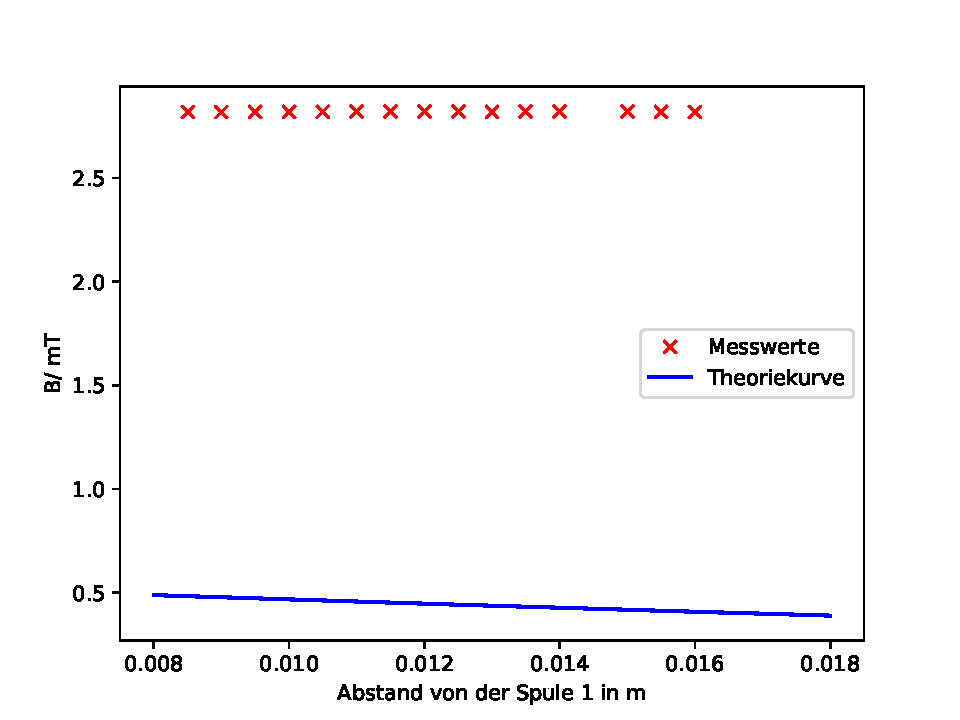
\includegraphics[height=8cm]{Helmholz1I.pdf}
  \caption{xB-Diagramm des Innenbereiches eines
  Helmholzspulenpaares im Vergleich zur Theoriekurve
  (I=2A).}
  \label{fig:Helmholz1I}
\end{figure}

\noindent Für die zweite Messreihe mit einer Stromstärke
von $I=5A$ wird äquivalent zur ersten Messreihe
vorgegeangen. Im folgenden sind die Messwerte sowie
die xB-Diagramme für den Außen- und Innenbereich
dargestellt.
\begin{table}[H]
  \centering
   \begin{tabular}{c c c c}
    \toprule
    Nummer der Oberwelle & $ U_{\text Theorie,Rechteck}\: / \si{\volt} $ &
    $ U_{\text Theorie,Dreick}\: / \si{\volt} $ & $ U_{\text Theorie,Sägezahn}\: / \si{\volt} $ \\
    \midrule
    1 & 1145 & 182 & 573 \\
    2 & 0 & 0 & 286 \\
    3 & 573 & 20 & 191 \\
    4 & 0 & 0 & 143 \\
    5 & 229 & 7 & 115 \\
    6 & 0 & 0 & 96 \\
    7 & 164 & 4 & 82 \\
    8 & 0 & 0 & 72 \\
    9 & 127 & 2 & 64 \\
    10 & 0 & 0 & 57 \\
    \bottomrule
  \end{tabular}
  \caption{Eingestellte Schwingungsamplituden.}
  \label{tab:tabe4}
\end{table}


\begin{figure}[H]
  \centering
  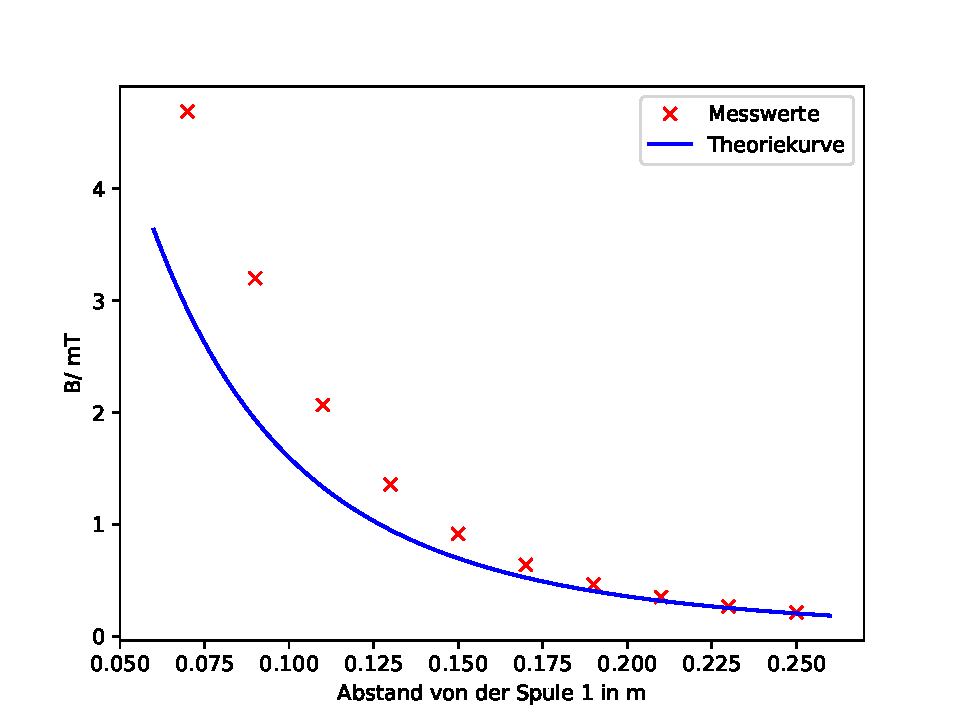
\includegraphics[height=8cm]{Helmholz2.pdf}
  \caption{xB-Diagramm des Außenbereiches eines
  Helmholzspulenpaares im Vergleich zur Theoriekurve
  (I=5A).}
  \label{fig:Helmholz2}
\end{figure}

\begin{figure}[H]
  \centering
  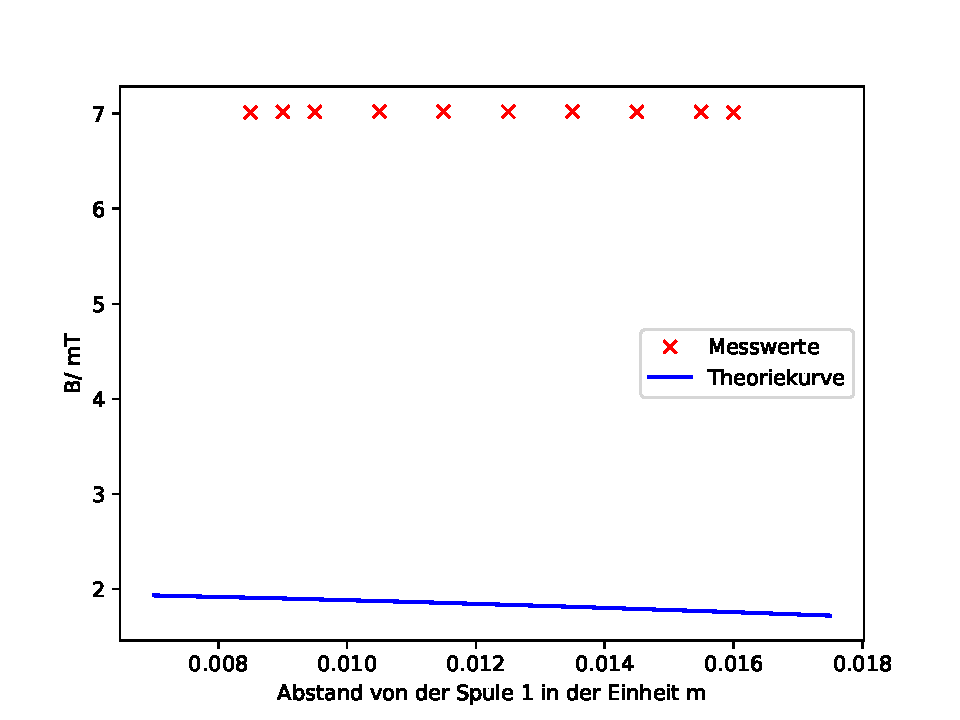
\includegraphics[height=8cm]{Helmholz2I.pdf}
  \caption{xB-Diagramm des Innenbereiches eines
  Helmholzspulenpaares im Vergleich zur Theoriekurve
  (I=5A).}
  \label{fig:Helmholz2I}
\end{figure}
\noindent An den Abbildungen \ref{fig:Helmholz1}
und \ref{fig:Helmholz2} wird deutlich sichtbar, dass
das Magnetfeld quadratisch abfällt und für große Abstände
gegen Null strebt. Dieses Ergebnis stimmt auch mit
der Formel \ref{eqn:inspule} überein. Jedoch weichen beide
Graphen für kleine Abstände von der Theoriekurve ab.
\noindent An den Messdaten sowie der Theoriekurve aus
Abbildung \ref{fig:Helmholz1I} und \ref{fig:Helmholz2I}
für den Innenbereich der Helmhozspulen wird deutlich, dass
das Magnetfeld in Inneren der Helmholzspulen
nahezu konstant ist. Doch beide Graphen liegen
deutlich unter der Theoriekurve.


\subsection{Magnetfeld von Spulen}
\noindent Die Aufgenommenen Messwerte für die kurze und lange
Spule sind in der folgenden Tabelle zu finden.
\begin{table}[H]
  \centering
  \caption{Wertetabelle für $\alpha$ und $C_V$.}
  \label{tab:tab2}
    \begin{tabular}{S S S S S}
    \toprule
    $ T\: \text{in}\: \si{\K} $ & $ {\alpha \cdot 10^{-6} \: \text{in}\: \si {\per\K}} $ &
    $ C_V \: \text{in}\: \si{\J\per\K\mol} $\\
    \midrule %Cv, a *10-6, Cv
    %0 & 1 & 1\\
    88.60\pm0.24 & 9.56\pm0.06 & 14.17\pm8.13  \\ %&3.6 & 318.97\pm0.85\\
    93.81\pm0.24 & 10.10\pm0.06 & 17.58\pm10.03 \\ %& 4.7 & 440.90\pm1.11\\
    99.74\pm0.24 & 10.66\pm0.05 & 15.52\pm8.84 \\ %& 5.1 & 508.68\pm1.21\\
    104.74\pm0.24 & 11.07\pm0.05 & 18.44\pm10.52 \\ %& 4.6 & 481.79\pm1.09\\
    110.94\pm0.24 &  11.54\pm0.05 & 14.86\pm8.45 \\ %& 5.3 & 587.97\pm1.27\\
    115.96\pm0.24 & 11.89\pm0.05 & 18.49\pm10.52 \\ %& 4.6 & 533.41\pm1.10\\
    121.47\pm0.24 &  12.22\pm0.05 & 16.83\pm9.57 \\ %& 4.9 & 595.21\pm1.17\\
    126.99\pm0.24 & 12.53\pm0.04 & 16.79\pm9.54 \\ %& 4.9 & 622.29\pm1.18\\
    131.58\pm0.24 & 12.77\pm0.04 & 20.42\pm11.62 \\ %& 4.2 & 552.62\pm1.01\\
    136.65\pm0.24 & 13.02\pm0.04 & 18.40\pm10.47 \\ %& 4.6 & 628.57\pm1.11\\
    141.49\pm0.24 & 13.24\pm0.04 & 19.28\pm10.97 \\ %& 4.4 & 622.54\pm1.07\\
    146.34\pm0.24 & 13.44\pm0.04 & 19.24\pm10.95 \\ %& 4.4 & 643.88\pm1.07\\
    150.95\pm0.24 & 13.62\pm0.04 & 20.22\pm11.52 \\ %& 4.3 & 649.11\pm1.05\\
    155.34\pm0.24 & 13.79\pm0.04 & 21.31\pm12.14 \\ %& 4.1 & 636.88\pm0.98\\
    159.97\pm0.24 & 13.95\pm0.04 & 20.12\pm11.47 \\ %& 4.3 & 687.89\pm1.05\\
    164.62\pm0.24 & 14.10\pm0.04 & 20.18\pm11.51 \\ %& 4.3 & 707.87\pm1.06\\
    168.79\pm0.25 & 14.23\pm0.04 & 22.54\pm12.86 \\ %& 3.9 & 658.27\pm0.95\\
    173.45\pm0.25 &  14.37\pm0.04 & 20.08\pm11.46 \\ %& 4.3 & 745.84\pm1.06\\
    178.13\pm0.25 &  14.50\pm0.04 & 20.04\pm11.44 \\ %& 4.3 & 765.94\pm1.06\\
    182.56\pm0.25 &  14.62\pm0.04 & 21.11\pm12.06\\
    192.70\pm0.25 &  14.87\pm0.04 & 18.41\pm10.47\\
    200.15\pm0.25 &  15.04\pm0.04 & 25.19\pm14.28\\
    208.87\pm0.25 &  15.23\pm0.04 & 21.43\pm12.18\\
    217.12\pm0.25 &  15.38\pm0.04 & 22.65\pm12.88\\
    225.15\pm0.25 &  15.53\pm0.03 & 23.27\pm13.24\\
    232.70\pm0.25 &  15.70\pm0.03 & 24.75\pm14.08\\
    240.53\pm0.25 &  15.74\pm0.03 & 23.84\pm13.58\\
    248.39\pm0.25 &  15.89\pm0.03 & 23.74\pm13.53& \\
    256.01\pm0.25 &  15.97\pm0.03 & 24.46\pm13.94 \\
    263.41\pm0.26 &  16.01\pm0.03 & 25.22\pm14.38 \\
    271.08\pm0.26 &  16.18\pm0.03 & 24.26\pm13.86 \\
    278.52\pm0.26 &  16.27\pm0.03 & 25.03\pm14.29&\\
    285.98\pm0.26 &  16.35\pm0.03 & 24.92\pm14.25 \\
    293.21\pm0.26 &  16.42\pm0.03 & 25.74\pm14.72 \\
    300.98\pm0.26 &  16.50\pm0.03 & 23.87\pm13.68 \\
    308.51\pm0.26 &  16.57\pm0.03 & 24.63\pm14.12\\



      \bottomrule
    \end{tabular}
\end{table}

Ähnlich zum Vorgehen bei den Helmhozspulen wird hier
ebenfalls ein xB-Diagramm erstellt, welches mit
der Theoriekurve
\begin{equation}
  B(z)=\frac{\mu_{0}nI}{2}\Biggl(\frac{z+(l/2)}{\sqrt{R^2+(z+(l/2))^2}}-\frac{z-(l/2)}{\sqrt{R^2+(z-(l/2))^2}}\Biggr)
  \label{eqn:inspule}
\end{equation}
verglichen wird. Es wird diese Formel zur berchnung der Theoriekurve verwendet, da
sich darüber sowohl das Magnetfeld im Inneren als auch im Außenbereich der
Spule berechenen lässt. Außerdem beziehen sich hier die
Abstände $z$ auf den Mittelpnkt der Spule, genau wie
die Messwerte auch.

\begin{figure}[H]
  \centering
  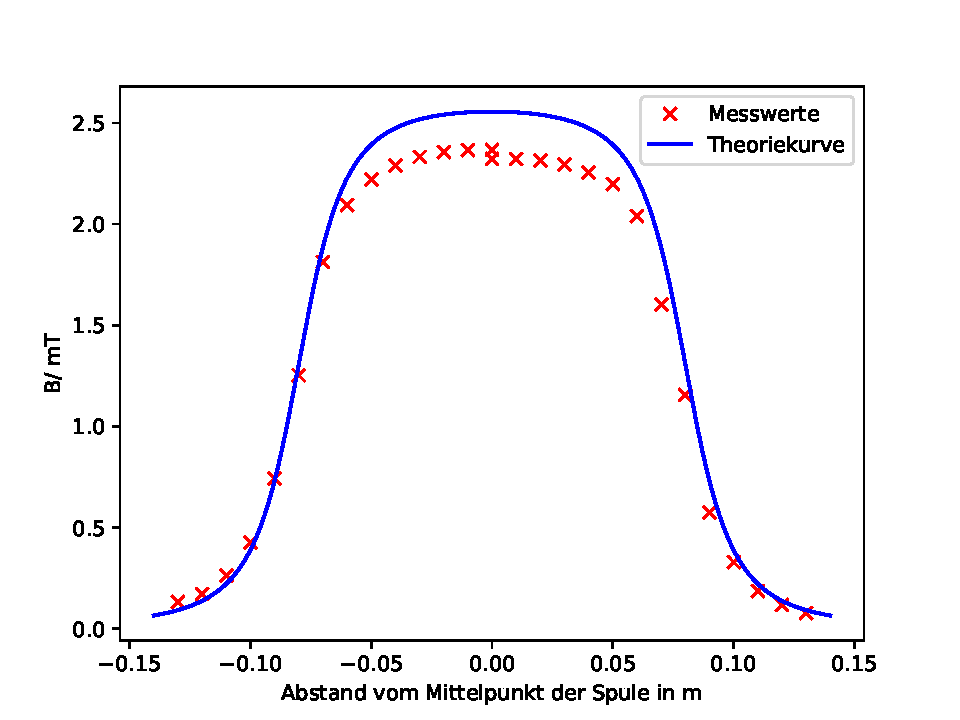
\includegraphics[height=8cm]{LangeSpule.pdf}
  \caption{xB-Diagramm der langen Spule.}
  \label{fig:LangeSpule}
\end{figure}
\begin{figure}[H]
  \centering
  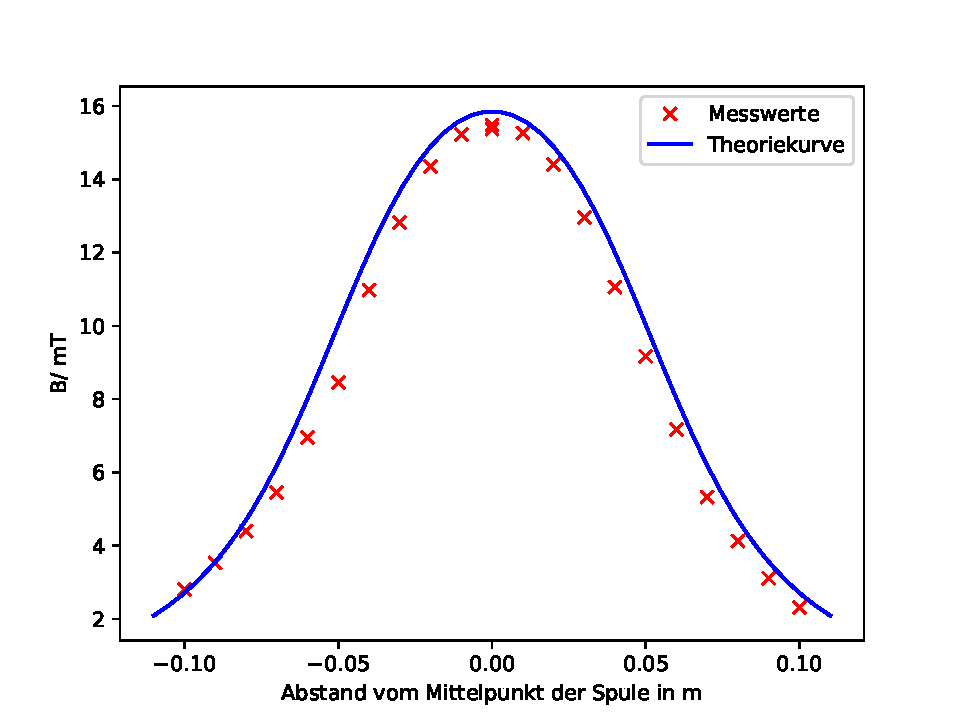
\includegraphics[height=7cm]{KurzeSpule.pdf}
  \caption{xB-Diagramm der kurzen Spule.}
  \label{fig:KurzeSpule}
\end{figure}

\noindent An den Abbildungen \ref{fig:LangeSpule} und \ref{fig:KurzeSpule}
wird deutlich, dass das Magnetfeld im Mittelpunkt
am stärksten ist, innerhalb der langen Spule ist es
sogar konstant. Nach außen hin fallen beide Felder
ab und streben für große Abstände gegen Null.



\label{sec:Auswertung}

%\begin{figure}
%  \centering
%  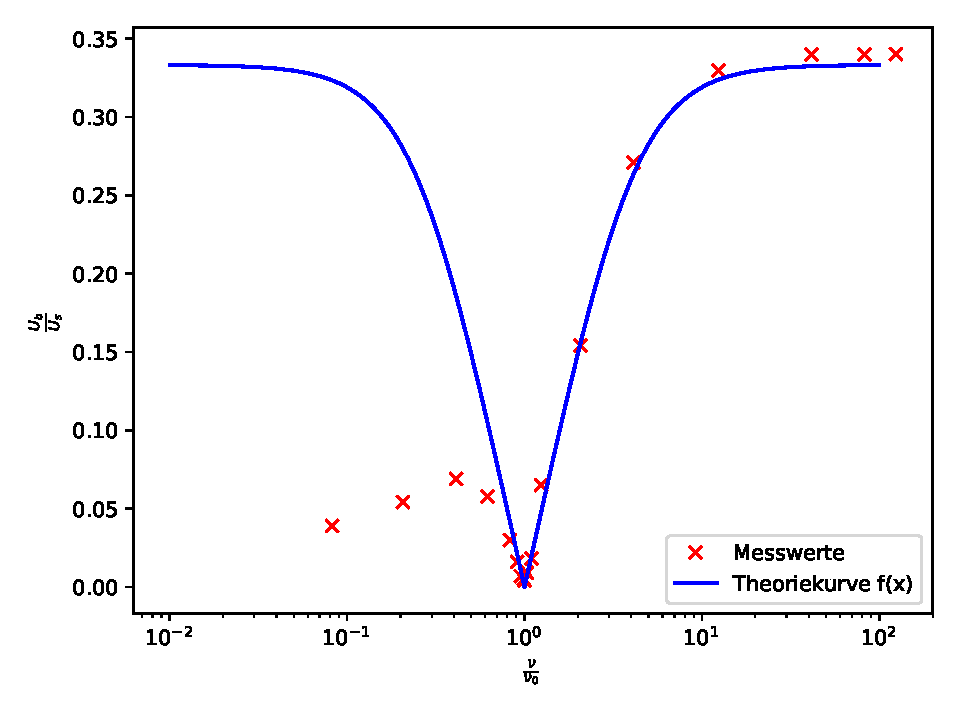
\includegraphics{plot.pdf}
%  \caption{Plot.}
%  \label{fig:plot}
%\end{figure}
